\documentclass[10pt,a4paper]{article}
\usepackage[utf8]{inputenc}
\usepackage{amsmath}
\usepackage{amsfonts}
\usepackage{amssymb}
\usepackage{multicol}
\usepackage{fullpage}
\usepackage{graphicx}
\usepackage{epstopdf}
\usepackage{cleveref}
\usepackage{float}
\usepackage{booktabs}
\usepackage{listings}
\usepackage{xcolor}
\usepackage[hidelinks]{hyperref}

\DeclareMathOperator\erf{erf}

\author{Daniel Underwood}
\title{Least Squares Curve Fitting}
\begin{document}

\definecolor{mygreen}{RGB}{28,172,0} % color values Red, Green, Blue
\definecolor{mylilas}{RGB}{170,55,241}

\lstset{language=Matlab,%
    %basicstyle=\color{red},
    breaklines=true,%
    morekeywords={matlab2tikz},
    keywordstyle=\color{blue},%
    morekeywords=[2]{1}, keywordstyle=[2]{\color{black}},
    identifierstyle=\color{black},%
    stringstyle=\color{mylilas},
    commentstyle=\color{mygreen},%
    showstringspaces=false,%without this there will be a symbol in the places where there is a space
    numbers=left,%
    numberstyle={\small \color{gray}},% size of the numbers
    numbersep=9pt, % this defines how far the numbers are from the text
    emph=[1]{for,end,break},emphstyle=[1]\color{red}, %some words to emphasise
    %emph=[2]{word1,word2}, emphstyle=[2]{style},    
}

\maketitle

\begin{multicols*}{2}
[
\section*{Linear Least Squares}
]

\subsection*{Background}

In linear least squares fitting, we have some set of data pairs $\{ (x_1, y_1), ... , (x_n, y_n)\}$ that we want to fit to an arbitrary function of the form

\begin{equation}
\sum\limits_i c_i f_i(x)
\label{eqn: arbitrary fit}
\end{equation}

A common form of curve fitting is to fit the data to a polynomial of order $m$. That is,

\begin{equation}
P_m(x) = \sum\limits_{k=0}^m c_k x^k
\label{eqn: general polynomial}
\end{equation}

In this report, we will fit $\erf{(x)}$, where $\erf{(x)}$ is the error function:

\begin{equation}
\erf{(x)} = \frac{2}{\sqrt{\pi}} \int\limits_0^x e^{-t^2} dt
\label{eqn: error function}
\end{equation}

It should be noted that least squares fitting is typically used to fit collected data to some function rather than generating points from an already-known function and trying to fit them.

\subsection*{Full Polynomial Fit}

First, we will fit $\erf{(x)}$ with a full polynomial. That is, a polynomial with powers such that every natural number less than $n$ is taken into account.

Plotted below are the errors of polynomial fits given by $\log \left| \erf{(x)} - P_m(x) \right|$ for a polynomial of order $m$. Plotted in this figure are polynomials with $m = 1, ..., 10$.

\begin{figure}[H]
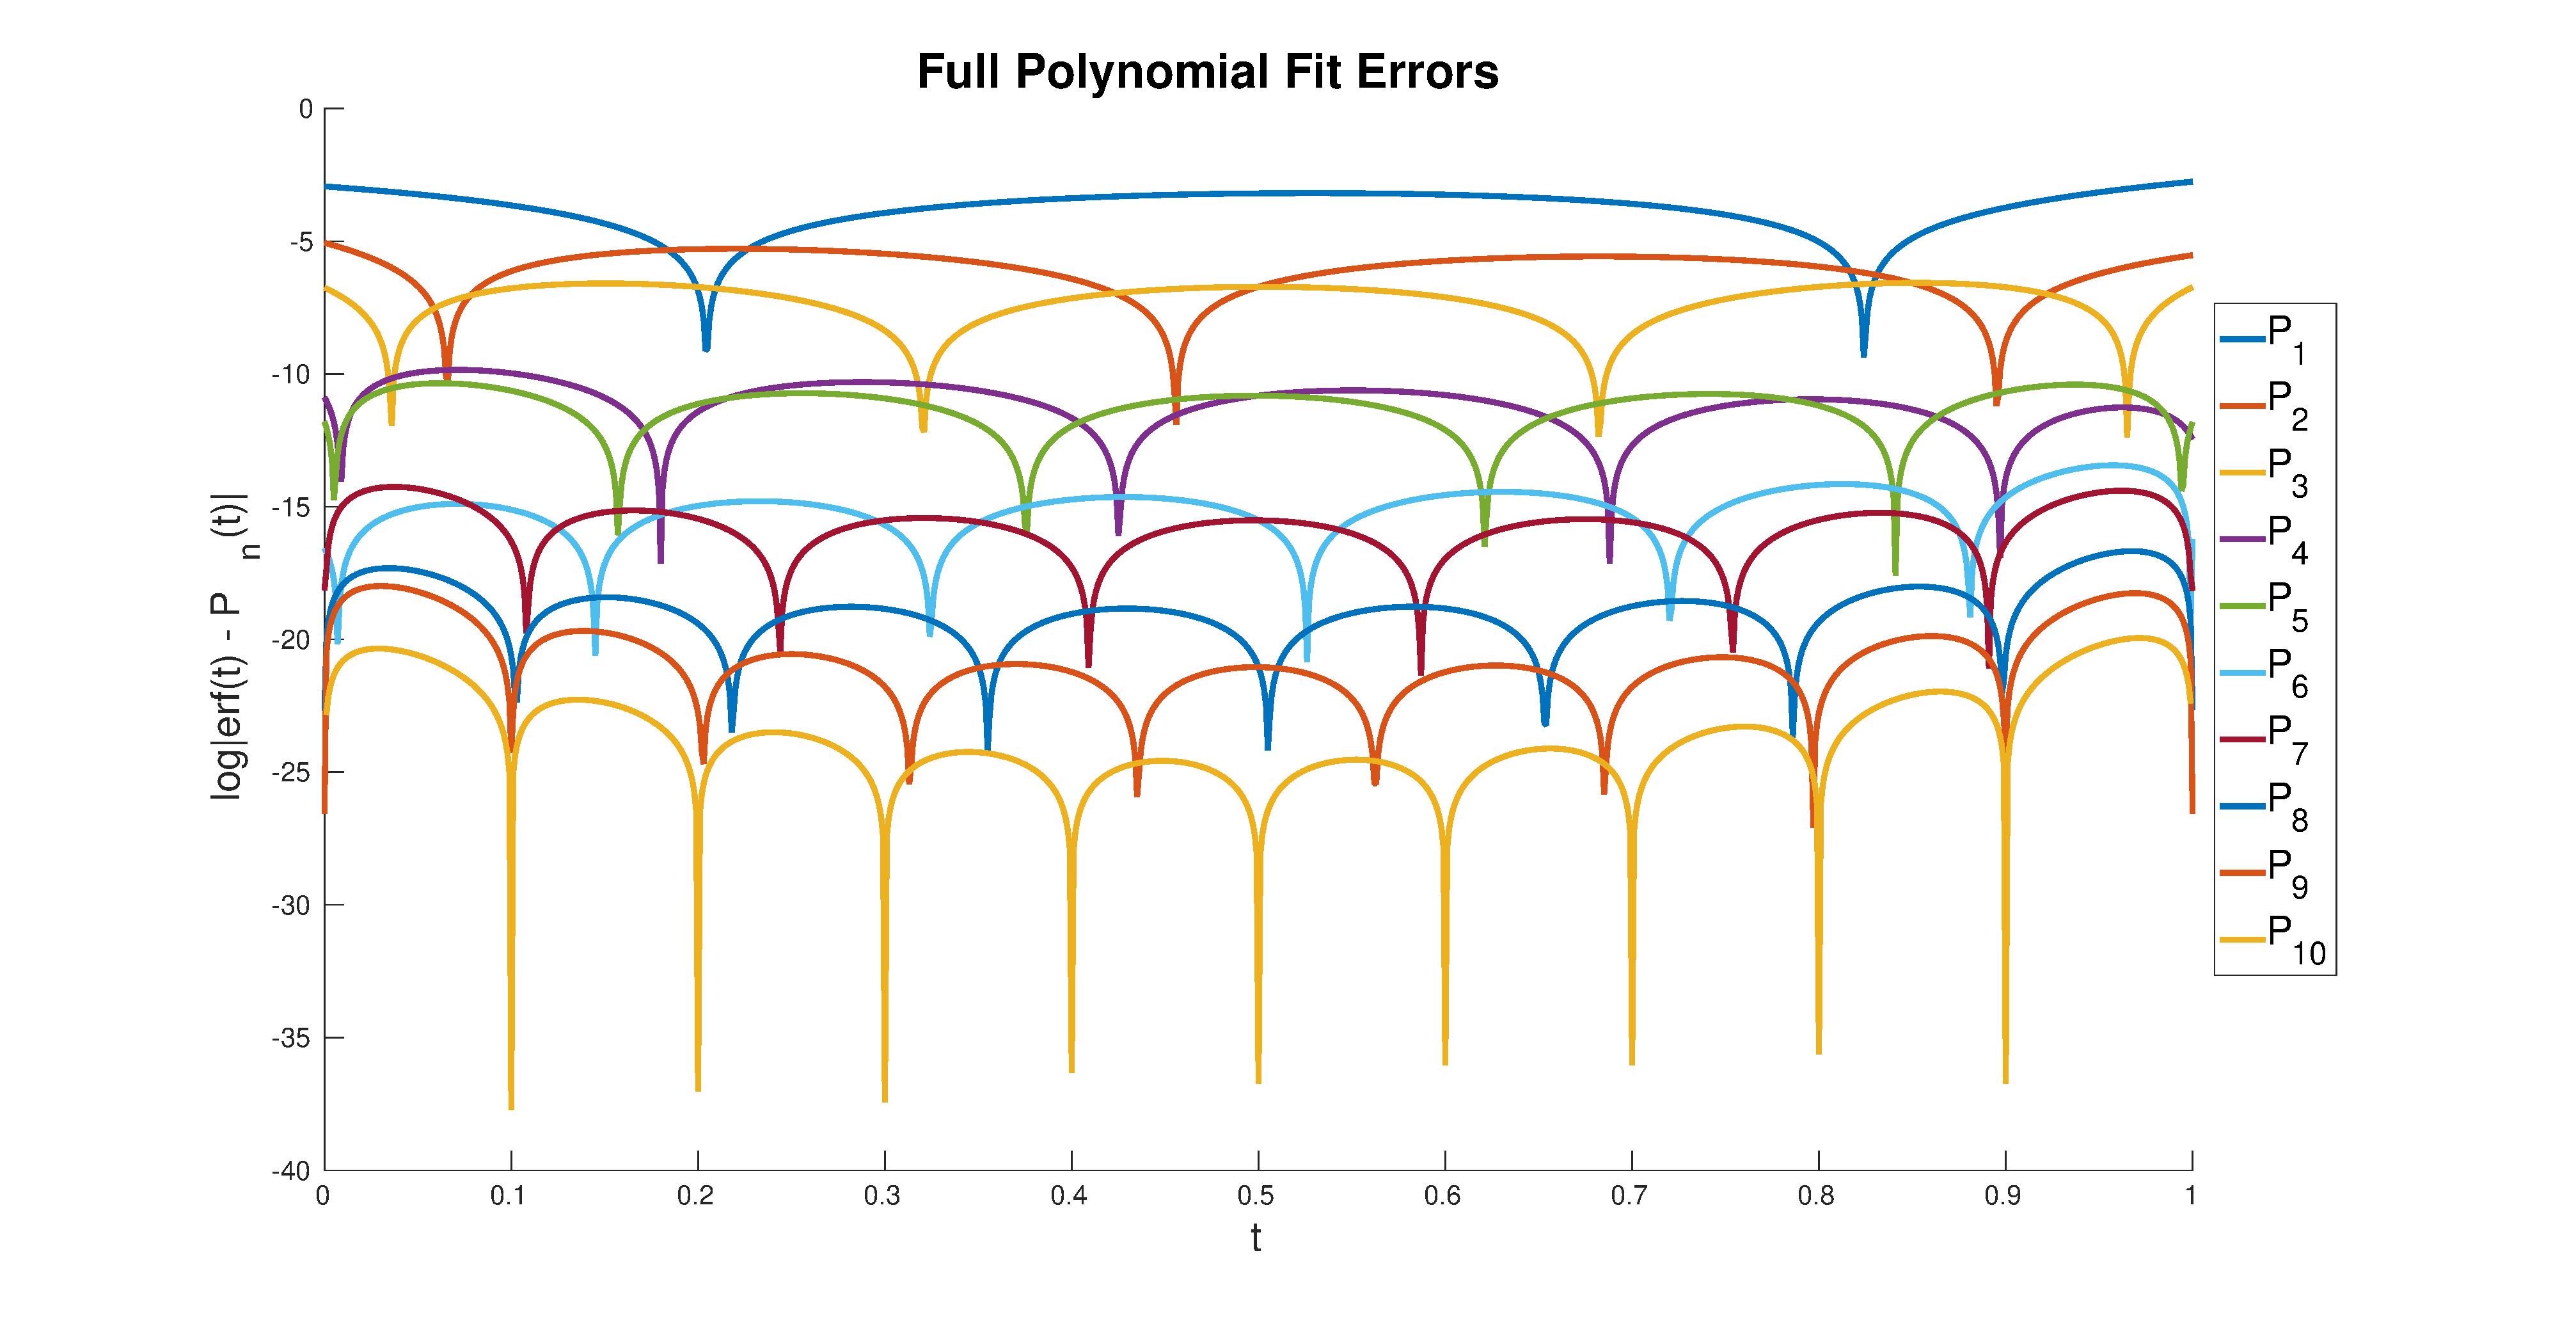
\includegraphics[width=\columnwidth]{Figures/fullpolyerror.eps}
\caption{Full Polynomial Fit Error Plot}
\label{fig: fullerror}
\end{figure}

As can be seen in \cref{fig: fullerror}, the error of the fits decreases as the order of the polynomial increases. This is expected as higher-order polynomials have more inflection points and can stay stable for a longer range before blowing up. It can also be noticed that all of the errors have approximate symmetry about $x=0.5$. In addition, the polynomials seem to be grouped closely into pairs of even and odd functions with a common error at $x=0.5$. Below is a table that tabulates the logarithm of the root mean squared error (RMSE) and the logarithm of the maximum absolute error for each degree of polynomial. Logarithms were used as the errors were too small on the interval $x \in [0,1]$ to be useful as decimals.

\begin{table}[H]
\begin{tabular}{l|rr}
\multicolumn{1}{l|}{} & \multicolumn{1}{c}{log(RMSE)} & \multicolumn{1}{c}{log(Max Absolute Error)} \\ \hline
$P_1$                  & -3.346804                     & -2.757447                                  \\
$P_2$                  & -5.639929                     & -5.060017                                   \\
$P_3$                  & -6.896321                     & -6.717131                                   \\
$P_4$                  & -10.759990                    & -9.974002                                    \\
$P_5$                  & -11.051908                    & -10.633327                                  \\
$P_6$                  & -14.866742                    & -14.178272                                  \\
$P_7$                  & -15.859004                    & -15.455704                                 \\
$P_8$                  & -19.275090                    & -18.750739                                \\
$P_9$                  & -21.709429                    & -21.044448                                 \\
$P_{10}$                 & -36.385632                    & -35.638188                                
\end{tabular}
\caption{Full Polynomial Fit Errors}
\label{table: fullerrors}
\end{table}

In \cref{table: fullerrors}, it is revealed that the error decreased as polynomial order increased, as seen in \cref{fig: fullerror}. From this, we can see that the RMSE and maximum absolute errors are relatively close, which indicates that most points have similar errors. It can also be seen that for $P_{10}(x)$, the RMSE and maximum errors are approximately $e^{-36} \approx 10^{-16}$, which is the maximum precision that is typically dealt with for a data type.

\subsection*{Odd Polynomial Fit}

In an effort to improve the fit to the error function points, other models are investigated. One thing quickly noticed is that since $\erf{(x)}$ is an odd function, it makes sense to fit the data to a purely odd polynomial. We will denote a purely odd polynomial as

\begin{equation}
O_j(x) = \sum\limits_{k=1}^j c_k x^k
\label{eqn: odd polynomial}
\end{equation}
Where $k$ must be odd. For this report, we will look at $j = 1, ..., 5$, resulting in polynomial degrees of 1 to 9.

Plotted below are the absolute errors of the purely odd polynomials. Once again, a logarithmic scale is used due to the low size of the errors.

\begin{figure}[H]
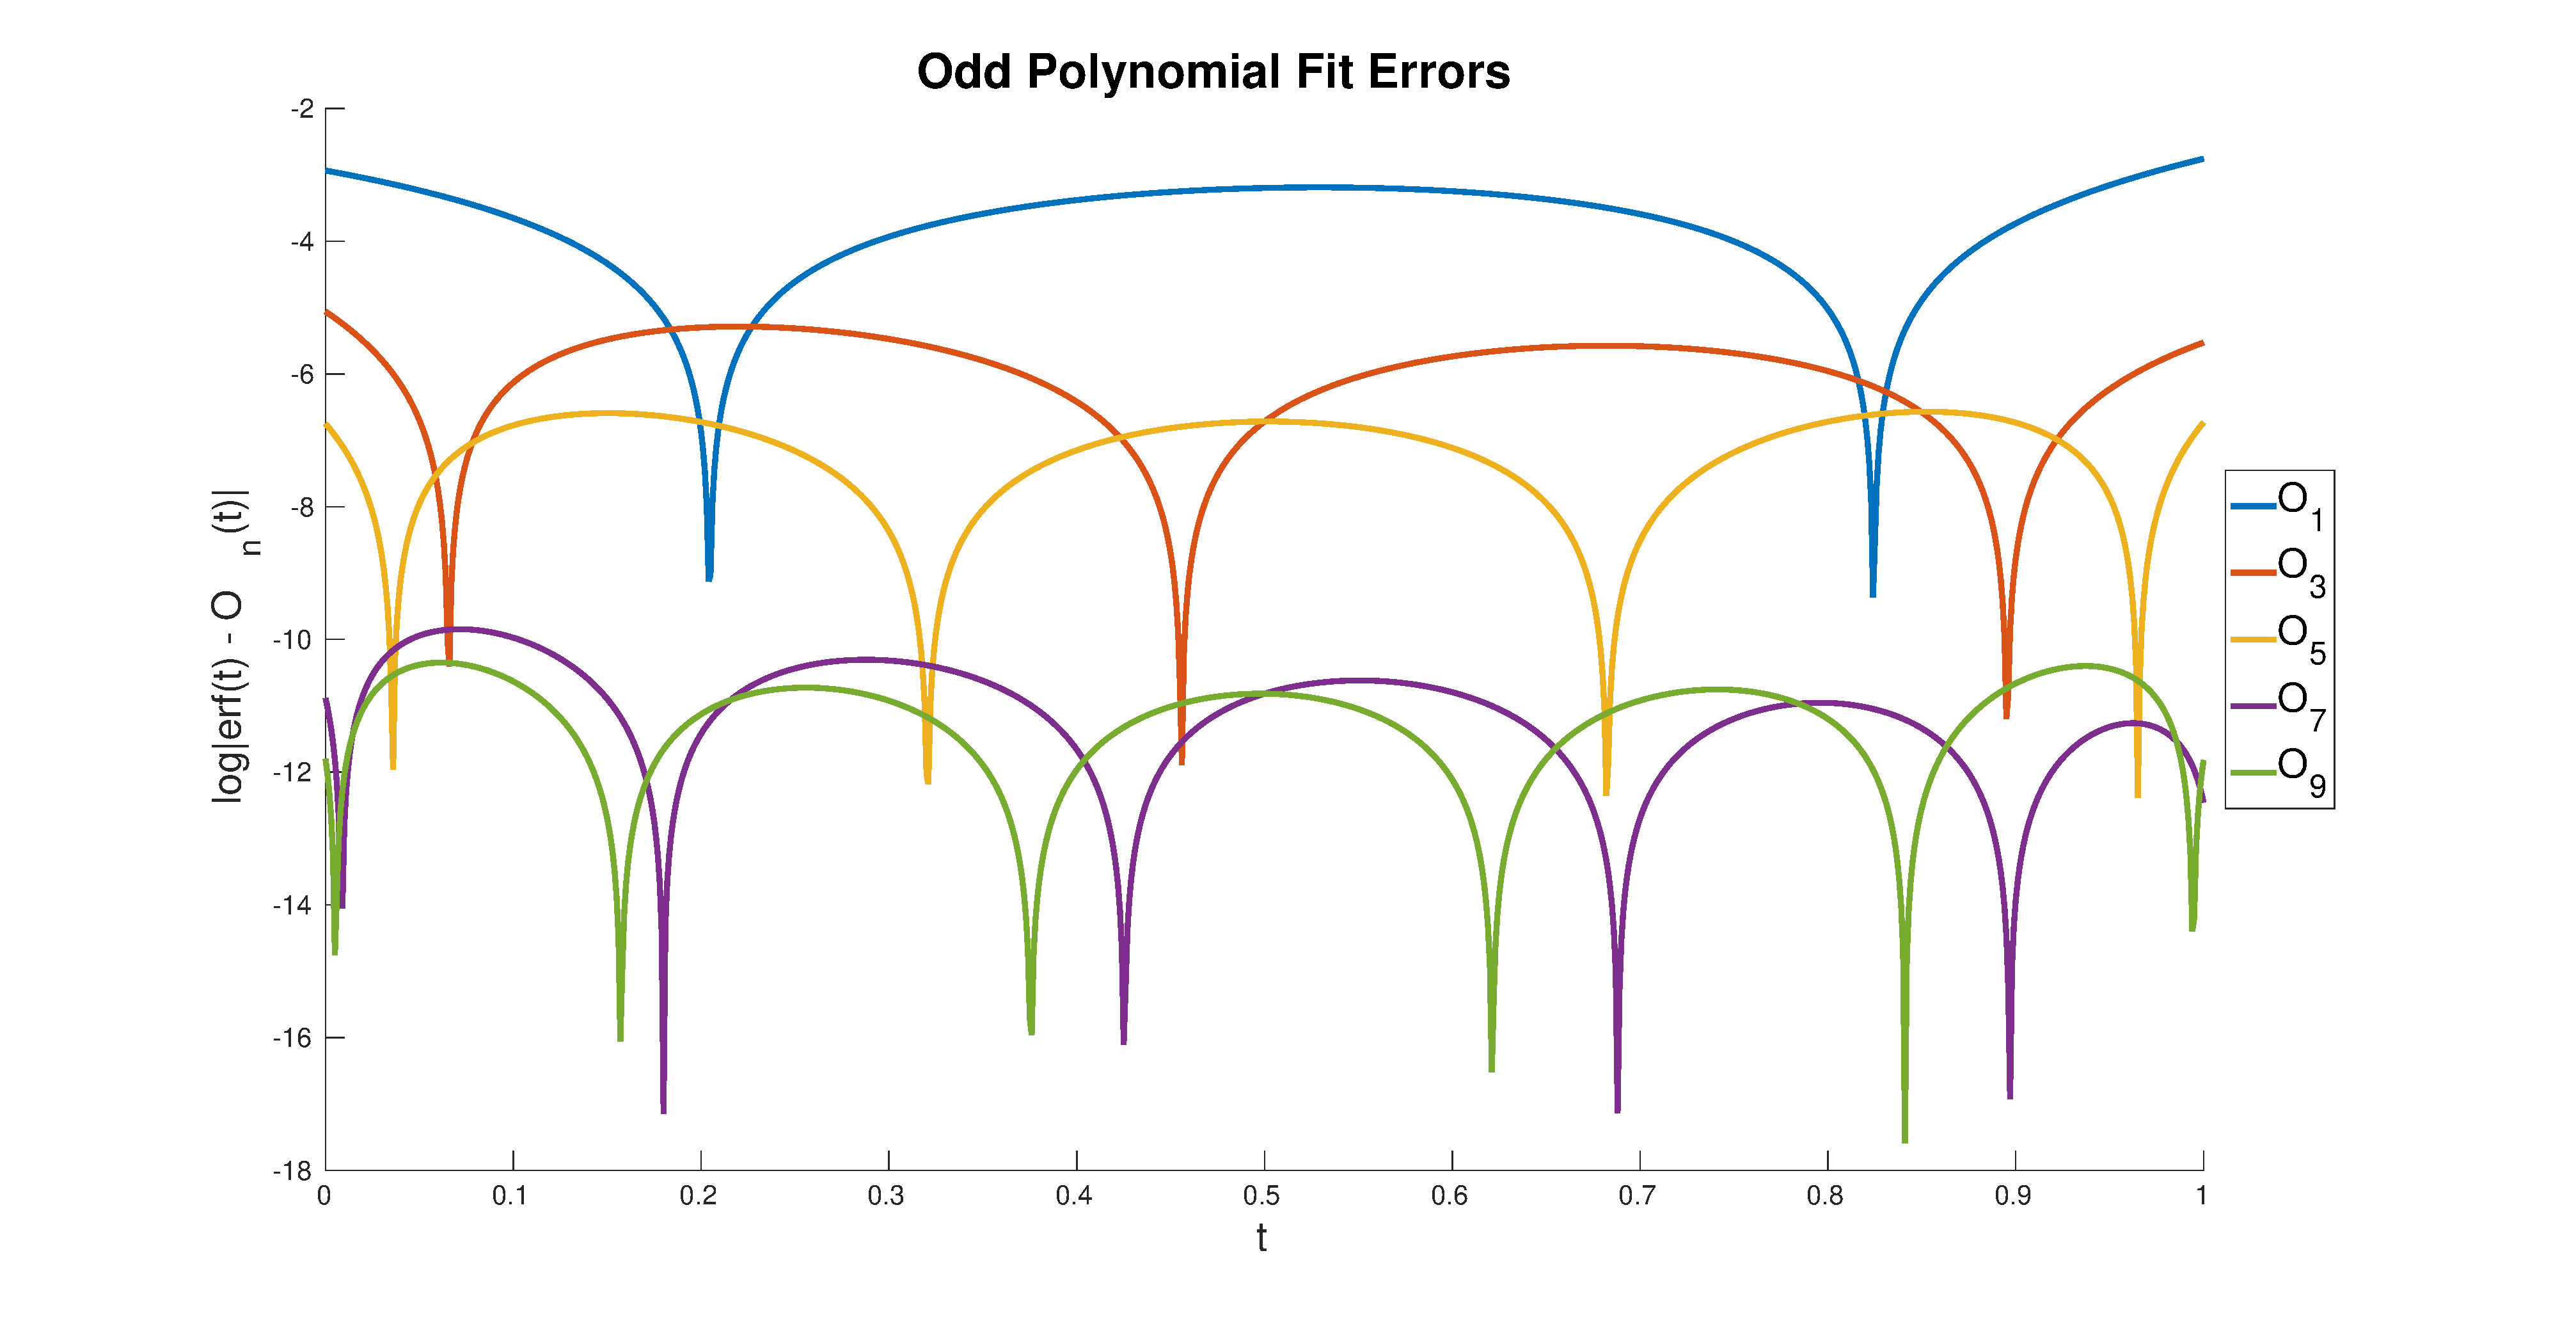
\includegraphics[width=\columnwidth]{Figures/oddpolyerror.eps}
\caption{Odd Polynomial Fit Error Plot}
\label{fig: odderror}
\end{figure}

It can be seen that the errors of the purely odd polynomials are unexpectedly larger than the full polynomials. While the exact cause of this is unknown, it is likely that the higher error is due to only looking at the error function evaluated on the interval $x \in [0,1]$ rather than an interval that includes negative values where the parity of the function would matter. The purely odd function would likely be an improvement if we looked at an interval such as $x \in [-1,1]$, although we will not examine such an interval here.

\begin{table}[H]
\begin{tabular}{l|rr}
     & \multicolumn{1}{c}{log(RMSE)} & \multicolumn{1}{c}{log(Max Absolute Error)} \\ \hline
$O_1$ & -3.096117             & -2.450822                           \\
$O_3$ & -5.678632            & -5.216506                           \\
$O_5$ & -8.521136            & -7.961519                           \\
$O_7$ & -11.631001           & -11.125641                          \\
$O_9$ & -15.013494             & -14.422444                          
\end{tabular}
\caption{Odd Polynomial Fit Errors}
\label{table: odderrors}
\end{table}

In \cref{table: odderrors}, the values of the logarithm of the RMSE and the max absolute error are listed for the purely odd polynomial. An interesting feature revealed is that the errors are similar to the corresponding full polynomial of order $\frac{j+1}{2}$ and being slightly more erroneous at lower orders and less so at higher orders. What this likely means is that since we are not looking at an interval where the function parity matters, only the number of times the function can ``twist'' matters, which is related to the number of terms in the polynomial. With a full polynomial, each term allows the function to change direction and become stable around a point. With the odd polynomial, there are only half as many terms, so there are fewer points at which the function can change from increasing to decreasing or decreasing to increasing.

\subsection*{Exponential Fit}

In search of a function that better fits the error function, it is necessary to look at some of the properties of the error function. One such property is the horizontal asymptote that the error function has. We know that $\lim\limits_{x \to \pm \infty} \erf{(x)} = \pm1$. This causes an issue with the models that we have been using as is is necessary for a polynomial of order greater than zero to have the property $\left| \lim\limits_{x \to \pm \infty} P_m(x)  \right| = \infty$. While the exact signs can vary based on the order of polynomial and the signs of its terms, a polynomial will most certainly never have a horizontal asymptote as $x \to \pm \infty$. To fit this property of the error function, we should choose a model that has a horizontal asymptote.

Of all elementary functions, the only nicely-behaved function that has a horizontal asymptote is the exponential decay. The exponential decay has a horizontal asymptote at $0$, although that can be changed to a constant by simply adding the constant as another term in the model. The problem arises that the rest of the exponential does not have the behavior that we see in the error function. We can solve this issue by using the product of the exponential decay and another function, which can also have a horizontal asymptote as the exponential term usually has more effect than other terms. The model that was chosen for this report is the following

\begin{equation}
c_1 + e^{-t^2} \left( c_2 + c_3 x + c_4 x^2 + c_5 x^3 \right)
\label{eqn: exponential model}
\end{equation}
where $x = \left( 1 + t \right)^{-1}$.

\begin{figure}[H]
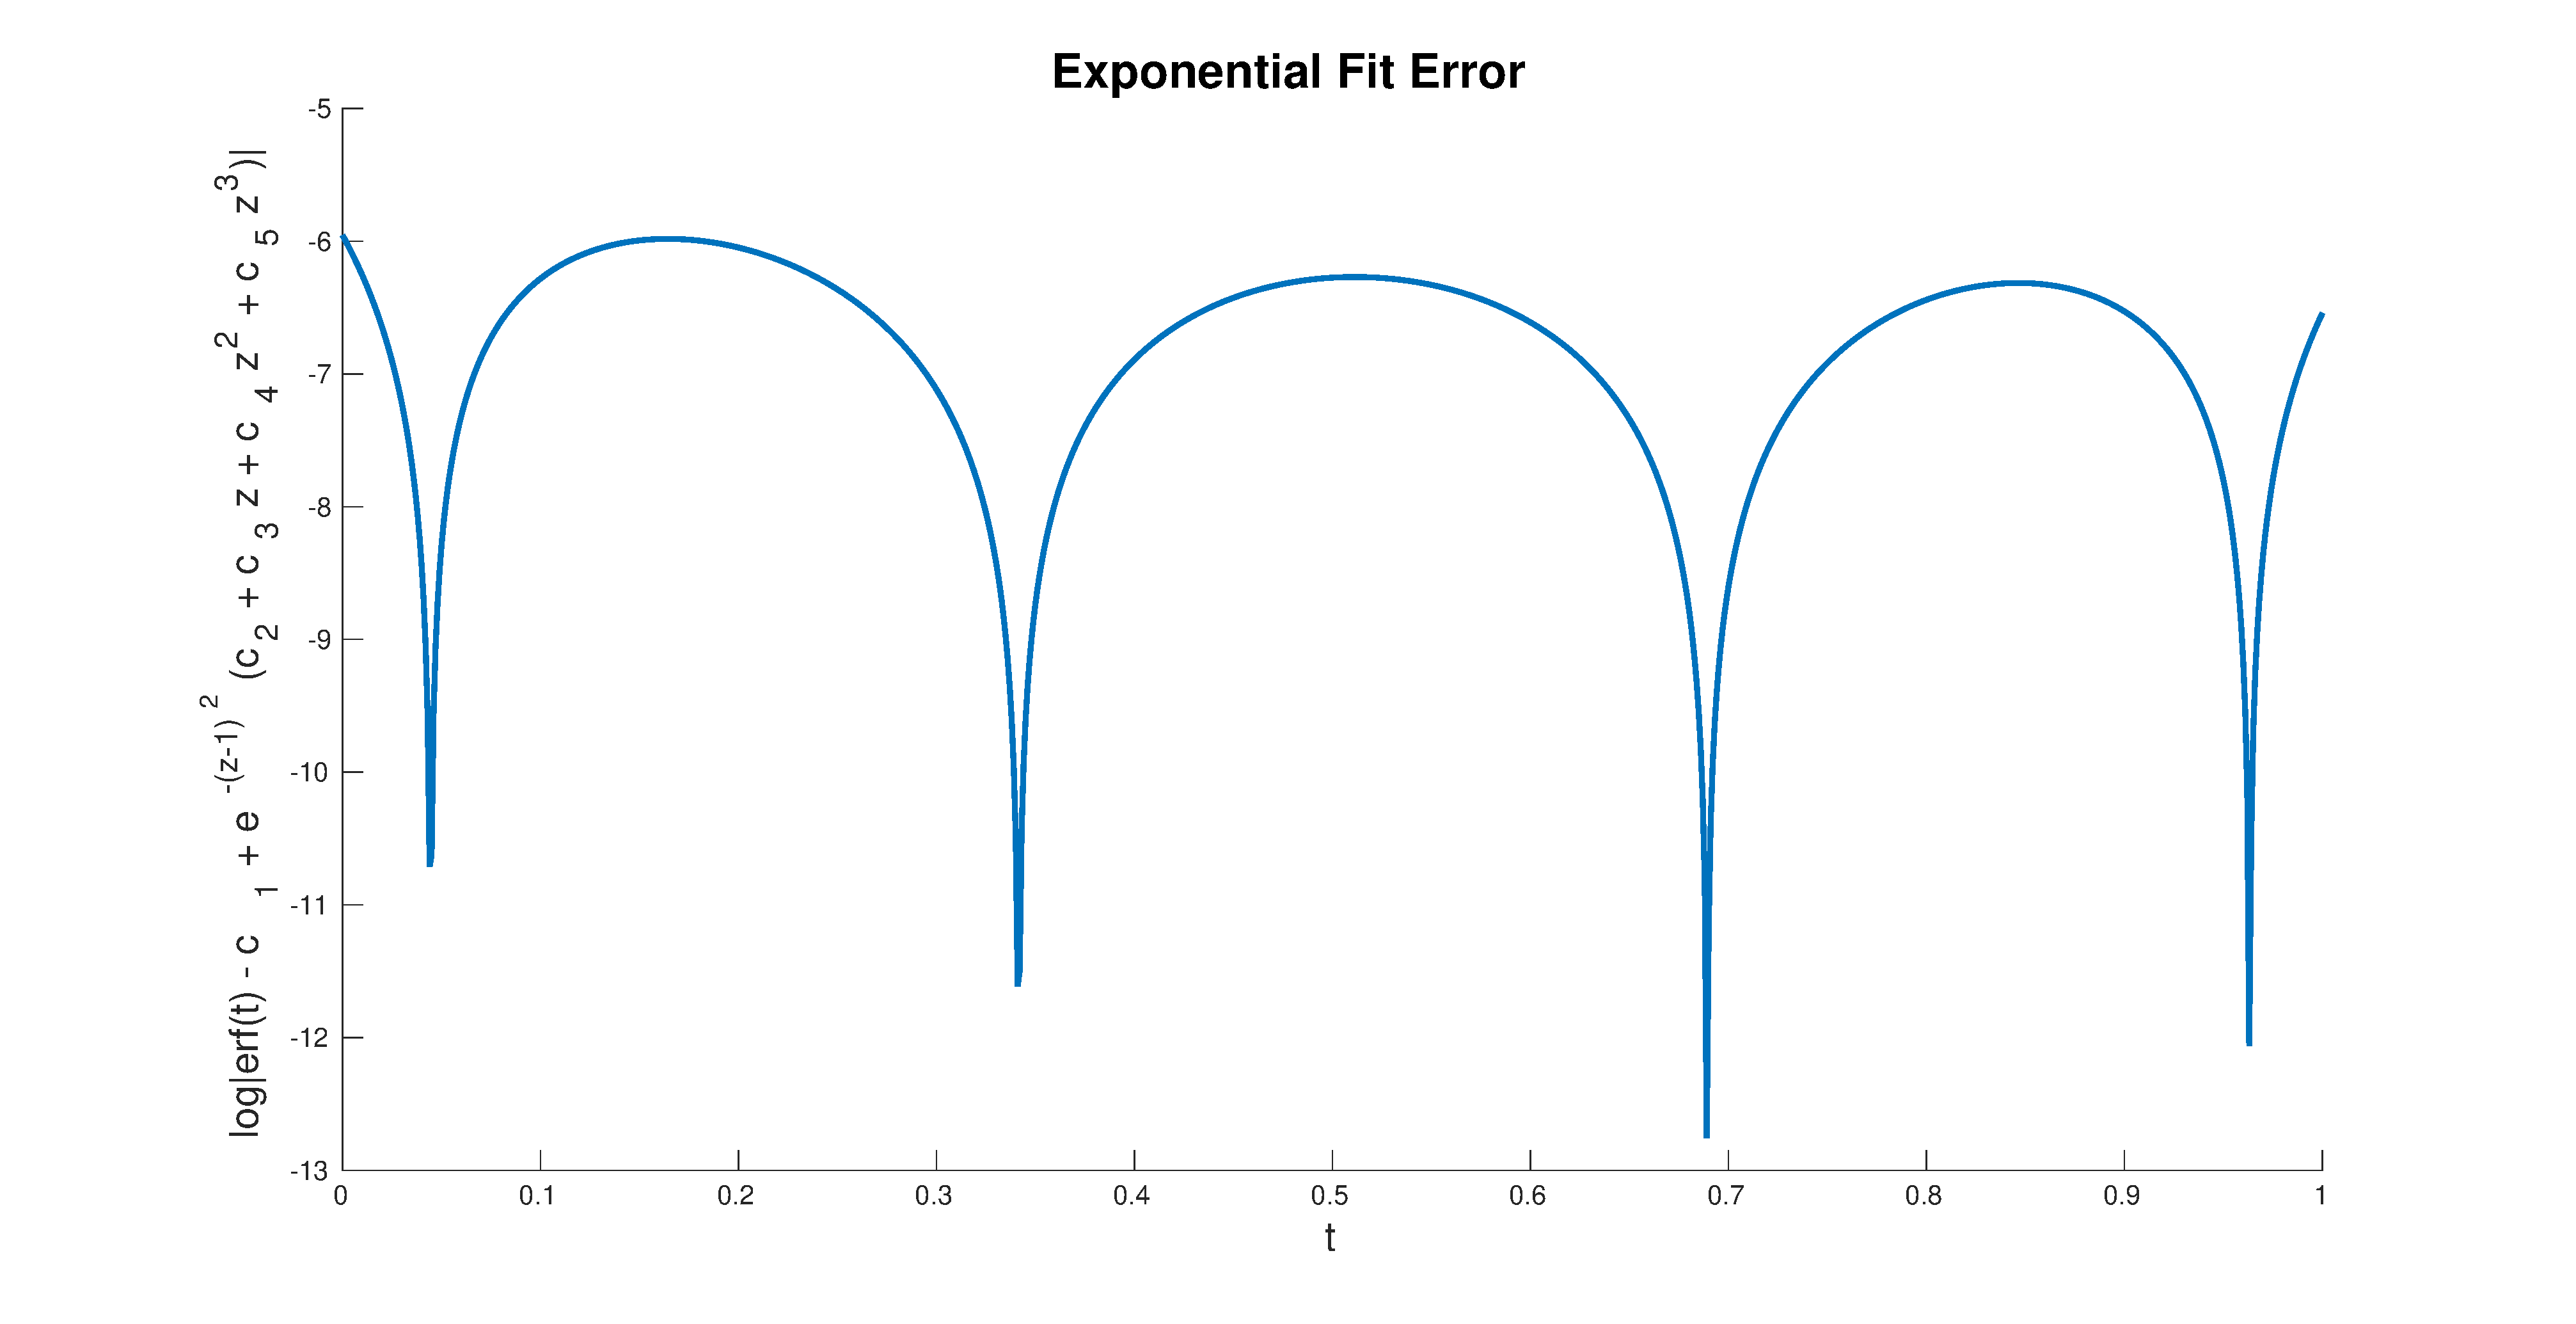
\includegraphics[width=\columnwidth]{Figures/experror.eps}
\caption{Exponential Fit Error Plot}
\label{fig: experrors}
\end{figure}

Plotted in \cref{fig: experrors} is the logarithm of the absolute error of the exponential fit to the error function. This is due to the asymptotic nature of the error function and the exponential; as $x$ increases, the error will decrease, with the hope that the error quickly becomes close to 0.

In addition, with this model, we found  the $\text{RMSE} \approx 0.076750$ and $\log{(\text{RMSE})} \approx -2.567242$. This model also resulted in a max absolute error of 0.170964 with a logarithm of -1.766301. Compared to the polynomials, these error values aren't great in the region of interest. However, the main feature of this model is the horizontal asymtote, which is important in the limits of the error function.

Additional improvements may be made by fitting a nonlinear model, resulting in parameters in places such as exponents.

\end{multicols*}

\begin{multicols*}{2}[ \section*{Nonlinear Least Squares} ]

\subsection*{Background}

In order to explore nonlinear least squares, we must have a nonlinear system. One such system is involved with determining the location of a GPS transmitter by satellite locations and signal transmission times using the navigation equation

\begin{equation}
\sqrt{ \left( x - x_i \right)^2 + \left( y - y_i \right)^2 + \left( z - z_i \right)^2 } - c \left( t_i - d \right) = 0
\label{eqn: navigationeqn}
\end{equation}
where $x_i$, $y_i$, $z_i$, and $t_i$ are respectively the $x$, $y$, and $z$ coordinates as well as transmittance time to satellite $i$. $x$, $y$, and $z$ are the spatial coordinates of the GPS transmitter and $d$ is the time error that the transmitter has. $c$ is the speed of light, which is approximately 299792.458 m/s.

\subsection*{4-Satellite GPS Problem}

Solving \cref{eqn: navigationeqn} requires at least 4 satellites to avoid having an infinite number of solutions. In fact, the case of four satellites results in a square system that can be reduced to a linear system. We will first solve for a system with the four satellites enumerated in the following table

\begin{table}[H]
\begin{tabular}{r|rrrr}
$i$ & \multicolumn{1}{c}{$x_i$} & \multicolumn{1}{c}{$y_i$} & \multicolumn{1}{c}{$z_i$} & \multicolumn{1}{c}{$t_i$} \\ \hline
1 & 15600                    & 7540                     & 20140                    & 0.07074                  \\
2 & 18760                    & 2750                     & 18610                    & 0.07220                  \\
3 & 17610                    & 14630                    & 13480                    & 0.07690                  \\
4 & 19170                    & 610                      & 18390                    & 0.07242                 
\end{tabular}
\caption{Satellites}
\label{table: satellites}
\end{table}

This system may be solved relatively simply with MATLAB's built-in \lstinline[language=matlab]|fsolve| function. This results in GPS transmitter values of 
$$
(x,y,z,d) = (-401.8, -16.8, 6370.1, 0)
$$

This location is very nearly the north pole, and is plotted in the following figure

\begin{figure}[H]
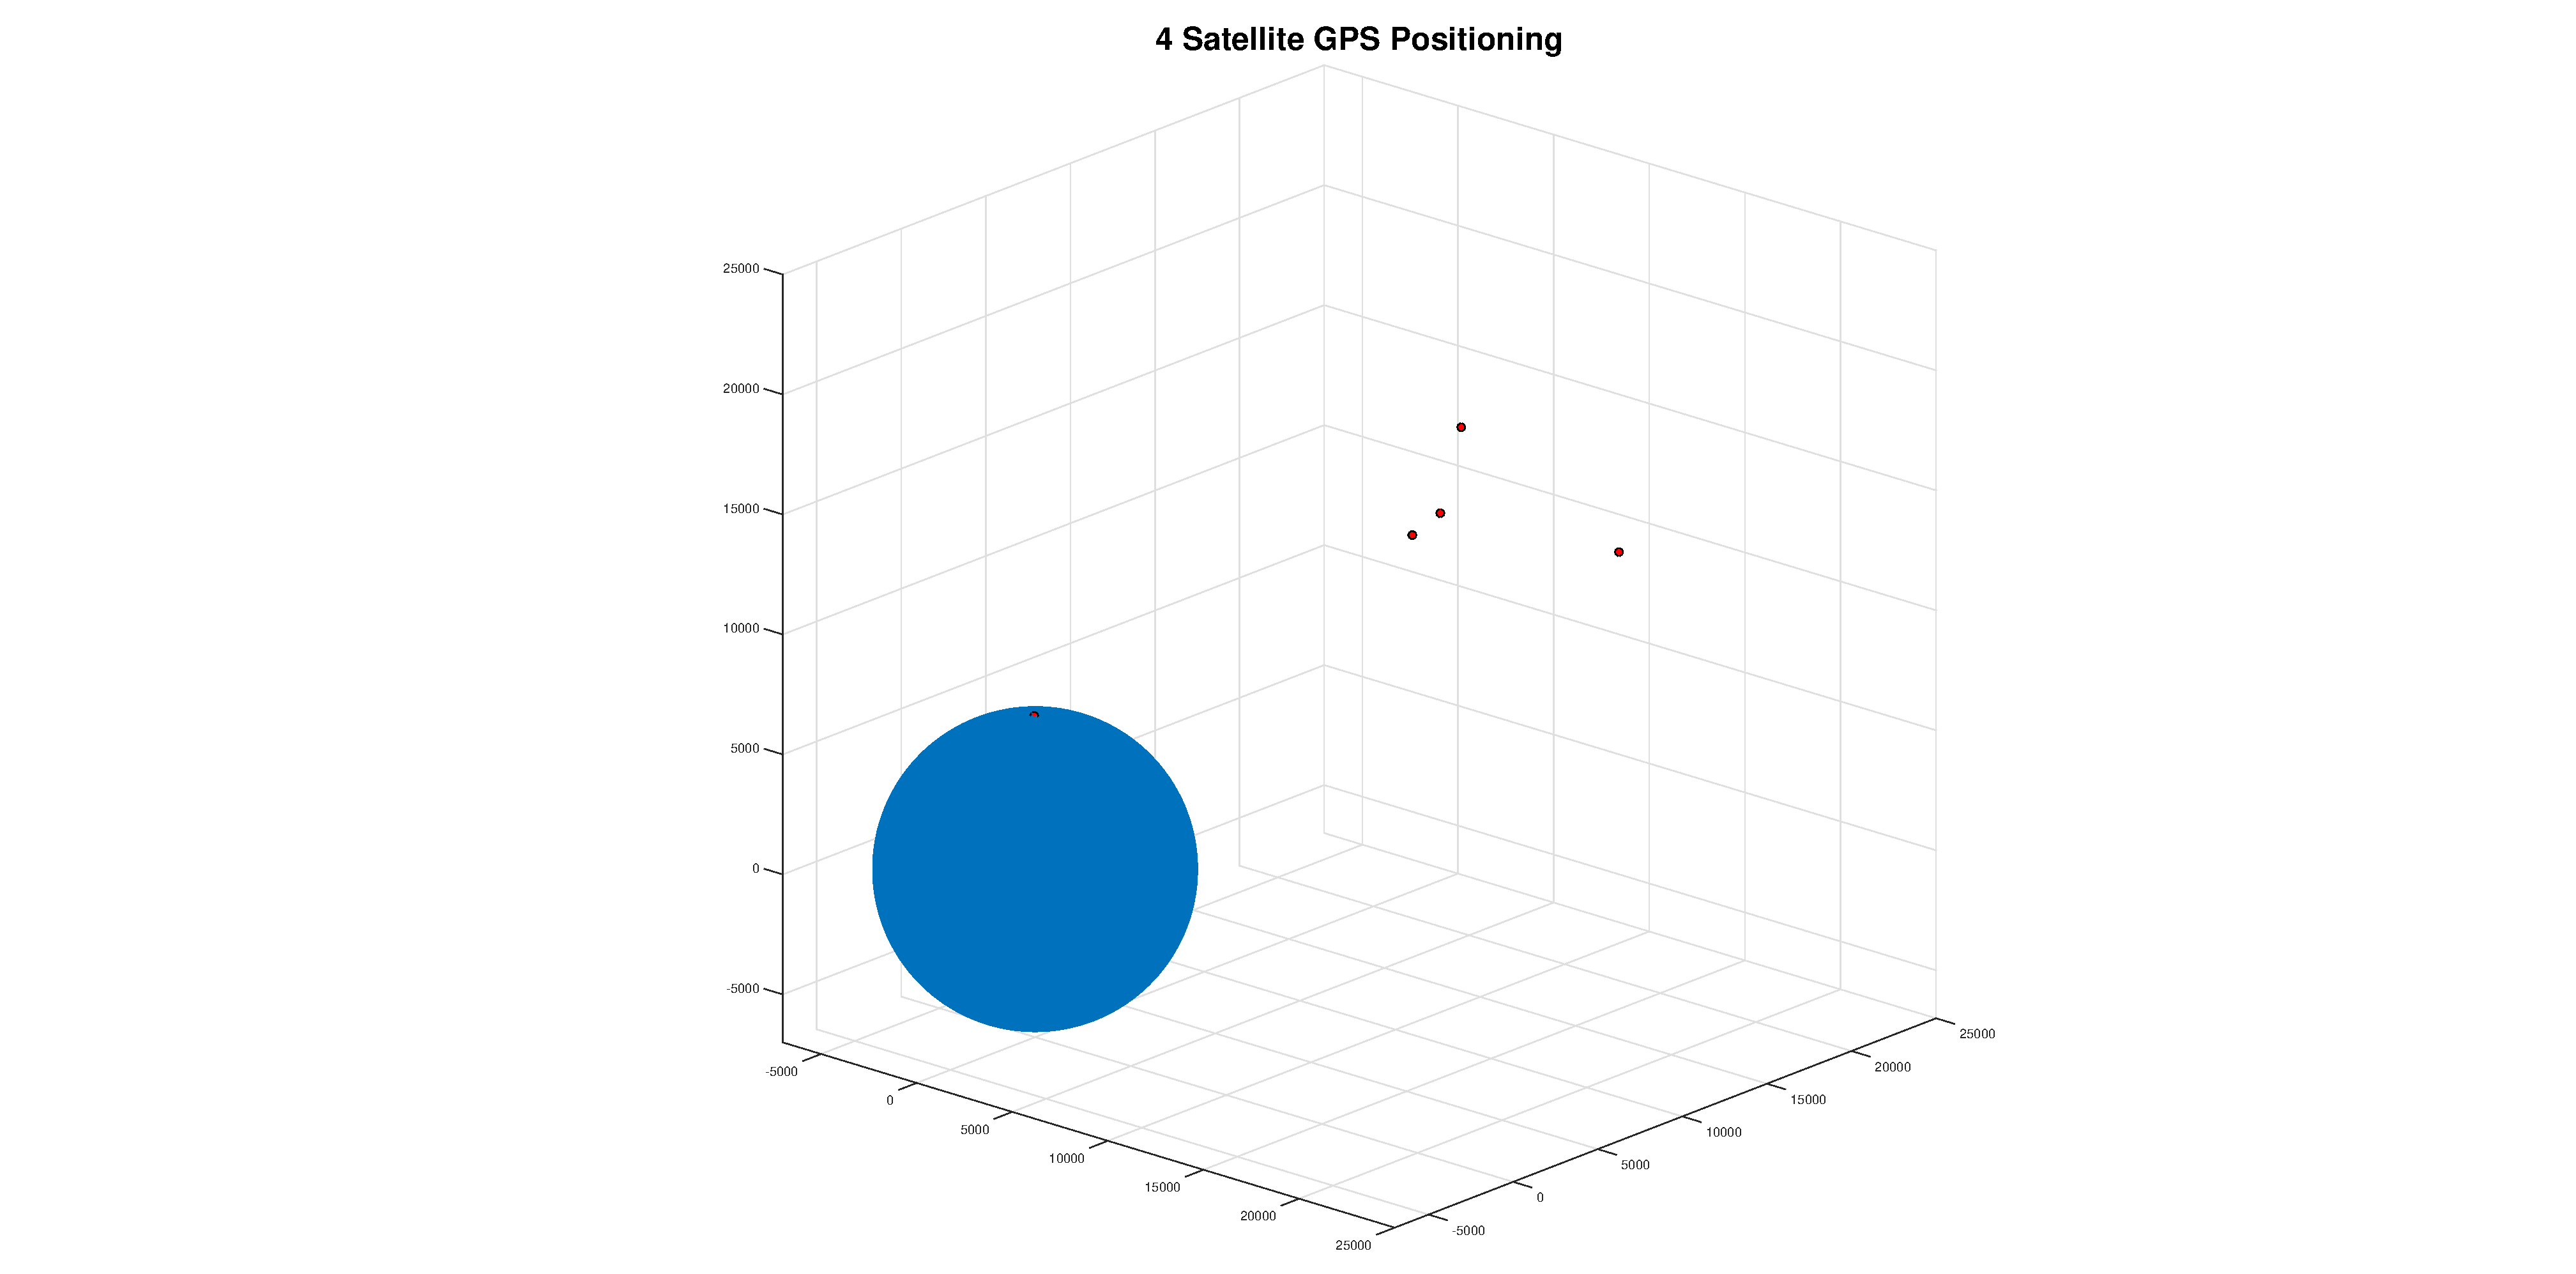
\includegraphics[width=\columnwidth]{Figures/4satgps.eps}
\caption{4-Satellite GPS System}
\label{fig: 4satgps}
\end{figure}

\subsection*{6-Satellite GPS Problem}

The GPS problem mentioned in the preceding sections may be made more interesting by involving more satellites. By increasing the number of satellites, the problem is no longer square and may be overdetermined; therefore, it is necessary to find a least-squares solution as an exact solution may not exist.

This case may be solved by MATLAB's \lstinline[language=matlab]|lsqnonlin| toolbox, which yields GPS transmitter values of
$$
(x, y, z, d) = (-10829, -4087, 1957, 0)
$$
As seen in the following plot, this would indicate that the transmitter is on the opposite side of the planet and is a good bit in the air

\begin{figure}[H]

\includegraphics[width=\columnwidth]{Figures/6satgps.eps}
\caption{6-Satellite GPS System}
\label{fig: 6satgps}
\end{figure}

The results shown in \cref{fig: 6satgps} is quite interesting as one would think that increasing the number of satellites would increase the accuracy of the measurement. This is in fact not the case since a least-squares result must be used. One suspected issue is the parameter $d$, which was found to be 0 in both the four and six-satellite cases. If $d$ were actually another number, it may be the case that both systems agree.
\end{multicols*}

\newpage

\section*{Source Code Listing}

In addition to the following source code listings, the newest versions of the code may be found at \url{https://github.com/danielunderwood/least-squares-curve-fitting} and the latest compiled version of this report may be found at \url{https://www.sharelatex.com/github/repos/danielunderwood/least-squares-curve-fitting/builds/latest/output.pdf}.
\lstinputlisting[language=matlab, caption=linlsqfit.m]{linlsqfit.m}
\lstinputlisting[language=matlab, caption=splitfunction.m]{splitfunction.m}
\lstinputlisting[language=matlab, caption=navigationequation4.m]{navigationequation4.m}
\lstinputlisting[language=matlab, caption=navigationequation6.m]{navigationequation6.m}
\end{document}